\subsection{Requirements and epic creation}
  The First stage is initiation, what's the project going to be about, how it fits into the company's strategy and OKRs, requirement gathering 
  and epic creation, an epic being a set of user stories/features (Karolis, Saulius, 2023).

  \begin{figure}[H]
    \centering
    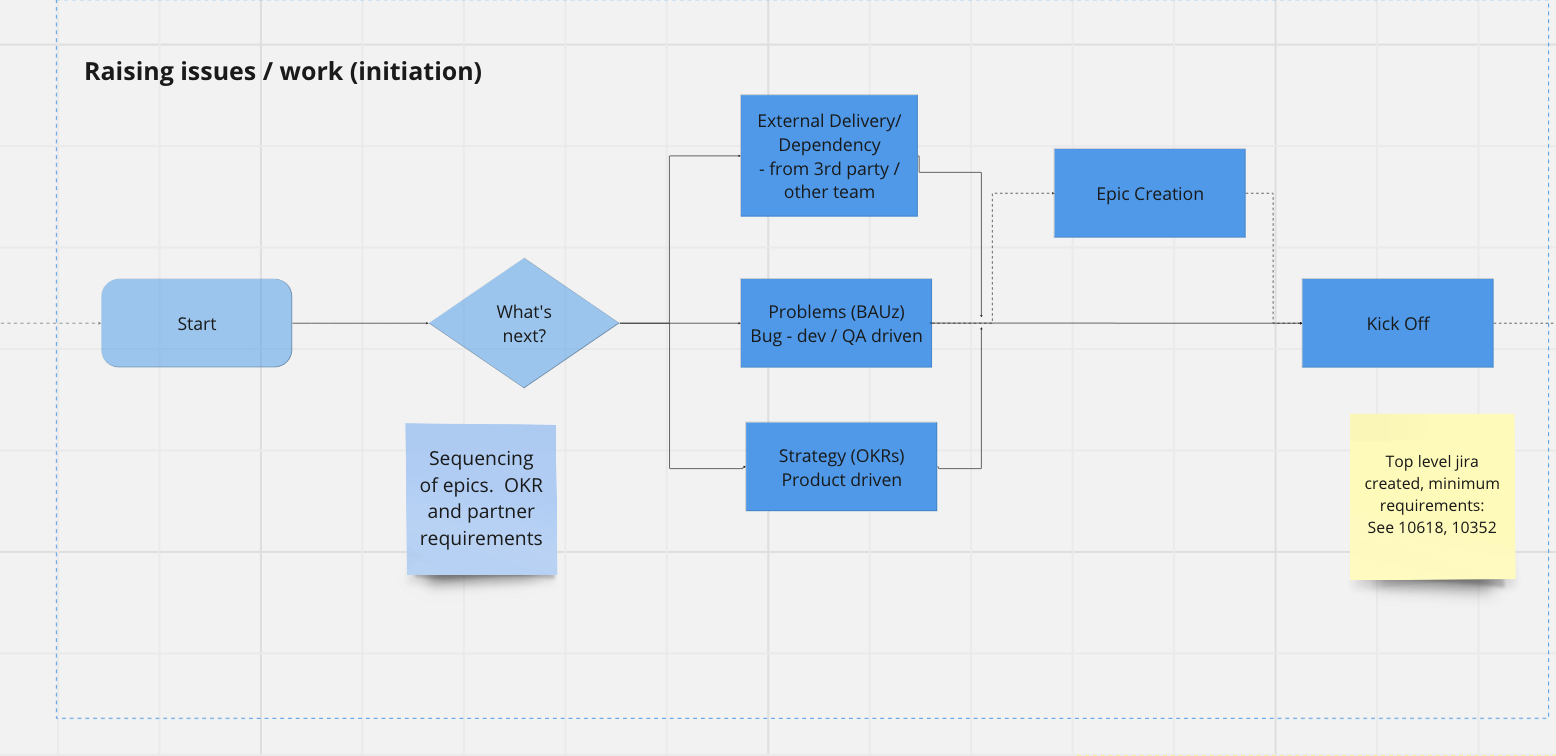
\includegraphics[width=8cm]{assets/workflow/initiate.png}
    \caption{Initiation stage of our ways of working.}
    \label{fig:workflowInitiate}
  \end{figure}

  Due to complications in project allocation, I was not involved in the initial phases of development for this project. However, discussions with 
  people that were, highlighted that due to the lack of external partner interaction there wasn't much to discuss and no solid requirements were 
  outlined, only the goal which is to allow the schedule generator to be moved from a static refresh of schedules to an event driven process.

  The benefits of the project and how it achieves our OKRs has been discussed previously in the report. However, I want to create some tangible
  requirements here using the MoSCoW framework which consists of must, should, could and won't haves (Eduardo, 2022). I will focus on software requirements and 
  denote whether they are functional (F) or non-functional (NF) (Bigelow 2020).

  \begin{enumerate}
    \item (F) The software \textbf{Must} be able to process schedule updates. 
    \item (F) The software \textbf{Must} be able to process episode updates.
    \item (F) The software \textbf{Must} be able to process ancestor updates.
    \item (NF) The software \textbf{Must} keep stored data more relevant than the static version.
    \item (F) The software \textbf{Must} still support a coldstart option.
    \item (F) The software \textbf{Must} contain alarms to alert us to errors.
    \item (F) The software \textbf{Should} gather metrics on processing time and types of updates.
    \item (F) The software \textbf{Should} clean up unneeded data from its store.
    \item (NF) The software \textbf{Could} support parallelised processing.
    \footnote{\textbf{SE-K02} - Although there were't any solid requirements captured by the team, I have broken down the project into its requirements
    to demonstrate what this could have looked like.}
    \footnote{\textbf{P5} - There were no external partners discussions for this project due to it being a change to an internal system. However, the
    following text simply describes this process and conflict management.}
  \end{enumerate}
  
  In this case requirement gathering was easy as there were no partners to discuss the changes with as it's all internal and the output to partners
  stays the same. If this wasn't the case, then requirements would have to be gathered from all partners affected or interested in the projects 
  outcome. These requirements would be gathered through meetings and conversations with these partners individually and compromises may have to 
  be made by both sides.
  This is usually the case when there is a requirement conflict, which can be described as:
  \begin{quote}
    \textit{'Requirements conflict is defined as unexpected or contradictory interaction between requirements that has a negative 
    effect on the results (Cameron, Velthuijsen, cited in Kim et al, 2007)'}
  \end{quote}
  These conflicts need to be managed well, as Kim et al (2007) warns these conflicts can \textit{'lead 
  to negative or undesired operation of the system'}. However certain stakeholders will often carry more leverage than another, taking into 
  consideration the Pareto Principle (Sanders, 1987), the 80-20 rule, it's easy for an organisation to leave out requirements of smaller stakeholders.
  A balance must be struck here where all parties are kept happy, without damaging the original idea of the project when large stakeholders try 
  and morph it into what they deem it should be.

  In this case no conflicts occurred due to the how internalised the project is. An epic was created in Jira and these requirements could then be explored 
  and implemented in the next phase.

\newpage